% Created 2012-09-08 Sat 22:11
\documentclass[11pt]{article}
\usepackage[utf8]{inputenc}
\usepackage[T1]{fontenc}
\usepackage{fixltx2e}
\usepackage{graphicx}
\usepackage{longtable}
\usepackage{float}
\usepackage{wrapfig}
\usepackage{soul}
\usepackage{textcomp}
\usepackage{marvosym}
\usepackage{wasysym}
\usepackage{latexsym}
\usepackage{amssymb}
\usepackage{hyperref}
\tolerance=1000
\usepackage[hmargin=2cm,vmargin=2.5cm]{geometry}
\usepackage{mathpazo}
\hypersetup{urlcolor=blue,colorlinks=true,linkcolor=red}
\setlength{\parskip}{0.5cm}
\setlength{\parindent}{0cm}
\setlength{\footnotesep}{0.25cm}
\usepackage{amsmath} \usepackage{mathtools}
\usepackage{cancel}
\providecommand{\alert}[1]{\textbf{#1}}

\title{Machine Learning, Prof. Andrew Ng}
\author{John W. Henderson}
\date{Last revised: \today}
\hypersetup{
  pdfkeywords={},
  pdfsubject={},
  pdfcreator={Emacs Org-mode version 7.8.03}}

\begin{document}

\maketitle

\setcounter{tocdepth}{4}
\tableofcontents
\vspace*{1cm}

\section{Week 1: Linear regression with one variable}
\label{sec-1}
\subsection{Terminology}
\label{sec-1-1}

Linear regression is the fitting of a line to a set of data in order to predict some
sort of mathematical relationship between the inputs (x's) and the output (y). These
\(x\)'s and \(y\)'s typically come in the form of ``training examples,'' which can be
thought of as ``rows'' of matched sets for data we already know.

The example used would be square area of homes \(x\)'s and corresponding sale prices
\(y\)'s. Machine learning aims to find a function to successfully predict new and
unknown output values given an input.

This function is known as the hypothesis, and is defined as \(h(\theta)\) where
\(\theta\) represents the parameters of our function. In the simplest case, we have a
single input, \(x\) and an output \(y\) and we want to fit a straight line to the
data in the form of \(y = mx + b\). Re-writing this equation in terms of \(\theta\),
we have \(h(\theta = \theta_0 + \theta_1 x\).

Given an input, \(x\) and values for \(\theta_0\) and \(theta_1\), we use the
hypothesis function to predict a new output value, \(y\).

Lastly, since we have multiple training examples, we use the notation \(x^{(i)}\) and
\(y^{(i)}\) to represent the \(i^{th}\) training example. \(m\) is used to denote the
number of training examples in the data.
\subsection{Cost function}
\label{sec-1-2}

In order to fit a hypothesis, we need to have a ``cost'' (or penalty) for incorrect
predictions, referred to as the cost function, \(J(\theta)\). For linear regression,
the mean sum of squared error function is sypically used:

\[
J(\theta) = \frac{1}{2m} \sum_{i=1}^m \left(h(x^{(i)}) - y^{(i)}\right)^2 = \frac{1}{2m}
\sum_{i=1}^m \left(\theta_0 + \theta_1 x^{(i)} - y^{(i)}\right)^2 
\]

In english this says, ``Take the output of my hypothesis function minus the actual
value for \(y\), square it, and then sum this value for all \(i\) of my training
samples. Lastly, divide by twice the number of my training samples.''
\subsection{Optimizing \(\theta\)}
\label{sec-1-3}


To find the best values for our \(\theta\)'s, we need to minimize our cost
function. This can be done by taking the derivative with respect to both \(\theta_0\)
and \(\theta_1\). This will involve the chain rule, which says:

\[
\frac{d}{dx} g(f(x)) = \frac{d}{df(x)} g(f(x)) \frac{d}{dx} f(x)
\]

In other words, take the derivative of \(g(x)\), treating \(f(x)\) like a variable
and multiply the result by the derivative of \(f(x)\), treating \(x\) like a
variable.

With that in mind, we can define our cost function in terms of \(g(f(\theta))\) and
\(f(\theta)\): 

\[
g(f(\theta)) = \frac{1}{2m} \sum_{i=1}^m \left(f(\theta)^{(i)}\right)^2 \\
\]
\[
f(\theta)^{(i)} = \theta_0 + \theta_1 x^{(i)} - y^{(i)}
\]

We need to find the derivatives with respect to both \(\theta\)'s. Starting with
\(\theta_0\), we'll take the partial of \(g(f(\theta))\):

\[
\frac{\partial}{\partial f(\theta_0)} g(f(\theta)) = \frac{\partial}{\partial
f(\theta_0)} \frac{1}{2m} \sum_{i=1}^m \left(f(\theta)^{(i)}\right)^2 =
\frac{1}{m} \sum_{i=1}^m f(\theta)^{(i)} 
\]

Since we're treating \(f(\theta)\) as the variable, \(g(f(\theta))\) is a simple
derivative in the form of \(\frac{d}{dx} x^2 = \frac{1}{2} x\).

Moving on to \(f(\theta)\), since we're taking the derivative with respect to
\(\theta_0\), \(\theta_1\), \(x\), and \(y\) are treated as constants \(\frac{d}{dx} c
= 0\).

\[
\frac{\partial}{\partial \theta_0} f(\theta)^{(i)} = \frac{\partial}{\partial
\theta_0} \theta_0 + \theta_1 x^{(i)} - y^{(i)} = 1 + 0 - 0 = 1 
\]

For the partial with respect to \(\theta_1\), \(g(f(\theta))\) is the same, but
\(f(\theta)\) now carries \(x^{(i)}\) through since \(\theta_1\) is the variable of
focus. Thus the partial is:

\[
\frac{\partial}{\partial \theta_1} f(\theta)^{(i)} = \frac{\partial}{\partial
\theta_1} \theta_0 + \theta_1 x^{(i)} - y^{(i)} = x^{(i)}
\]

Combining our definitions, we have:
\[
\frac{\partial}{\partial \theta_0} g(f(\theta)) = \frac{1}{m} \sum_{i=1}^m
f(\theta)^{(i)} \frac{\partial}{\partial \theta_0} f(\theta)^{(i)} = \frac{1}{m} \sum_{i=1}^m f(\theta)^{(i)} \times 1  = \frac{1}{m} \sum_{i=1}^m \left(\theta_0 + \theta_1 x^{(i)} -
y^{(i)}\right)
\]

And,
\[
\frac{\partial}{\partial \theta_1} g(f(\theta)) = \frac{1}{m} \sum_{i=1}^m
f(\theta)^{(i)} \frac{\partial}{\partial \theta_1} f(\theta)^{(i)} = \frac{1}{m}
\sum_{i=1}^m f(\theta)^{(i)} \times x^{(i)}  = \frac{1}{m} \sum_{i=1}^m
\left(\theta_0 + \theta_1 x^{(i)} - y^{(i)} \right) x^{(i)}
\]

These partial derivatives allow us to find the point at which our cost function is
minimized; namely, the point \((\theta_0, \theta_1)\) where
\(\frac{\partial}{\partial \theta_0, \theta_1} J(\theta) = 0\). 
\subsection{Gradient descent}
\label{sec-1-4}


To find this optimized point minimizing \(J(\theta)\), we can use an algorithm called
gradient descent, which increments our values for \(\theta\) along the function
\(J(\theta)\) toward the direction where it flattens out at a minima. The mean
squared error function produces a derivative function shaped like a parabola (one
variable) or bowl (multiple variables). Since this is the case, linear regression has
no local minima, only one global minima. As we move away from the minima in one
direction, slope will be positive; in the other direction it will be negative. To
move toward the minima, we can use the update rule:

\[
\theta_0 := \theta_0 - \alpha \frac{1}{m} \sum_{i=1}^m \left(\theta_0 + \theta_1
x^{(i)} - y^{(i)} \right)
\]
\[
\theta_1 := \theta_1 - \alpha \frac{1}{m} \sum_{i=1}^m \left(\theta_0 + \theta_1
x^{(i)} - y^{(i)} \right) x^{(i)}
\]

\(\alpha\) is known as the \emph{learning rate} and determines how far in the direction of
the minima we should step. If one steps in very small increments, it can be shown
that the algorithm will necessarily converge on the minima, but at the cost of a high
number of gradient descent iterations. If \(\alpha\) is too large, however, gradient
descent can fail to converge. One step will overshoot the minima and end up on the
opposing side of the parabola. At this new point, the slope of the parabola is larger
(with the opposite sign) and so the next iteration will overstep the minima by an
even larger amount. This will cause the algorithm to diverge further and further from
minimizing \(J(\theta)\).

The suggested remedy for this is to start with a small value of \(\alpha\) and
monitor \(J(\theta)\) for a continual decrease after every iteration of gradient
descent. A suggested starting value for \(\alpha\) is \(0.01\). One can increase by
\(3 \times \alpha\) until a balance is reached between rapid convergence and minimal
increase in hypothesis error.
\section{Week 2: Regression with multiple features}
\label{sec-2}
\subsection{Redefinining \(h(\theta)\) and gradient descent}
\label{sec-2-1}

We can also apply linear regression to multiple features. To re-use the housing price
example, instead of only predicting on the square area, perhaps we want to improve
our hypothesis by taking into account the number of bedrooms, number of bathrooms,
and the age of the house. For this larger array of values:

\begin{itemize}
\item \(x^{(i)}\) still denotes the \(i^{th}\) training set (rows)
\item \(x_j\) is the vector for the \(j^{th}\) feature (columns)
\item \(x^{(i)}_j\) is the \(j^{th}\) feature (column) of the \(i^{th}\) training example (row)
\end{itemize}

We get a table like this for our features/training examples:

\(
\begin{array}{c|c|c|c|c}
x_1 & x_2 & x_3 & ... & x_n \\
\hline
x^{(1)}_1 & x^{(1)}_2 & x^{(1)}_3 & \vdots & x^{(1)}_n \\
x^{(2)}_1 & x^{(2)}_2 & x^{(2)}_3 & \vdots & x^{(2)}_n \\
\vdots & \vdots & \vdots & \vdots & \vdots \\
x^{(m)}_1 & x^{(m)}_2 & x^{(m)}_3 & \vdots & x^{(m)}_n \\
\end{array}
\)

Extending the original definition of \(h(\theta)\), we now have
\[
h(\theta) = \theta_0 + \theta_1 x_1 + \theta_2 x_2 + ... + \theta_n x_n
\]

If we insert a left-most column, \(x^{(i)}_0\) where all training example values for
feature \(x_0\) are equal to 1, we can re-write the equation like this:
\[
h(\theta) = \theta_0 x_0 + \theta_1 x_1 + \theta_2 x_2 + ... + \theta_n x_n
\]

If we take the derivative with respect to any \(\theta_n\), we have:
\[
\frac{1}{m} \sum_{i=1}^m \left(h(\theta) - y^{(i)} \right) x^{(i)}_j
\]

This function serves as a universal cost function derivative equation since \(x_0 =
1\). The partial with respect to \(\theta_0\), then, is exactly as we derived it
above with only one feature.

Our generalized gradient descent algorithm becomes:
\[
\theta_j = \theta_j - \alpha \frac{1}{m} \sum_{i=1}^m \left(h(\theta) - y^{(i)} \right) x^{(i)}_j 
\]
\subsection{The vectorized regression model}
\label{sec-2-2}


We can view our \(x\)'s as a matrix (table), and \(\theta\)'s as a vector
(column). Since matrix multiplication multiplies the elements of every row, \(j\),
of one matrix by every column, \(i\), of another matrix, we can re-write
the hypothesis function in vectorized form:
\[
h(\theta) = X \theta
\]

\(X\) will be an \(m \times n\) matrix and \(\theta\) will be an \(n \times 1\)
matrix; the product will yield an \(m \times 1\) matrix where every element, \(X
\theta^{(i)}\) is equal to:
\[
X \theta^{(i)} = \theta_0 x^{(i)}_0 + \theta_1 x^{(i)}_1 + ... + \theta_n x^{(i)}_n
\]

In vectorized form, the cost function can be written as:
\[
J(\theta) = \frac{1}{m} \sum_{i=1}^m \left( X \theta^{(i)} - Y^{(i)} \right)^2
\]
\subsection{Feature scaling}
\label{sec-2-3}

When using multiple features, gradient descent can be quite slow to find the values
of \(\theta\) that minimize the cost function if features are not on the same order
of magnitude. An example would be predicting the selling price of a house based on
square footage (\(900 <= x_1 <= 4,000\)), age (\(5 <= x_2 <= 100\)) and number of
bed/bathrooms (\(1 <= x_3 <= 5\)). In these types of situations it is helpful to both
normalize and center the feature vectors.

To accomplish this, two practices are common. The first is to scale each feature so
that all of the features are in ranges of the same order of magnitude. A common
practice is to scale them to \(0 <= x <= 1\) by dividing each training example from a
given feature vector by the range for that feature's values:
\[
x^{(i)}_{j-scaled} = \frac{x^{(i)}_{j}}{x_{j-max} - x_{j-min}}
\]

Another commonly used denominator is the standard deviation for that feature.


The second practice is centering the data around the mean by subtracting
the mean from each training sample value for that feature. In other words:
\[
x^{(i)}_{j-scaled} = x^{(i)}_{j} - \frac{1}{m} \sum_{i=1}^m x^{(i)}_j
\]

Combined, we can scale data with either of the following methods:
\[
x^{(i)}_{j-scaled} = \frac{x^{(i)}_{j} - \mu_{x_j}}{range_{x_j}} \textrm{ \qquad or \qquad } 
x^{(i)}_{j-scaled} = \frac{x^{(i)}_{j} - \mu_{x_j}}{\sigma_{x_j}}
\]
\subsection{The normal equation}
\label{sec-2-4}

Instead of iterating through gradient descent, it is possible to mathematically find
the values of \(\theta\) that minimize the cost function. This is known as the normal
equation, and is defined as:
\[
\theta = \left( X^T X \right)^{-1} X^T Y
\]

In terms of evaluating whether to use the normal equation or gradient descent:

\begin{itemize}
\item Gradient descent:
\end{itemize}


\begin{center}
\begin{tabular}{{p{0.4\textwidth}lp{0.4\textwidth}}}
 \textbf{Pros}         &     &  \textbf{Cons}         \\
\hline
 - Will find solution, even for very large number of features (\(n >= 200,000\))  &     &  - Slow; requires a lot of iterations, especially for small \(\alpha\) or large data sets  \\
 - Will find solution if \(X^T X\) ends up being non-invertable (very small likelihood)  &     &  - Need to pre-scale feature vectors and pre-scale prediction inputs  \\
                       &     &  - \(\alpha\) value might cause divergence  \\
\end{tabular}
\end{center}



\begin{itemize}
\item Normal equation
\end{itemize}

\begin{center}
\begin{tabular}{{p{0.4\textwidth}lp{0.4\textwidth}}}
 \textbf{Pros}         &     &  \textbf{Cons}         \\
\hline
 - Faster than gradient descent  &     &  - High computing cost (\(O^3\))  \\
 - No risk of poor choice of \(\alpha\)  &     &  - Very slow for large number of features \((n >= ~10,000\))  \\
 - No need to scale features  &     &                        \\
\end{tabular}
\end{center}
\section{Week 3: Logistic regression}
\label{sec-3}
\subsection{Classification}
\label{sec-3-1}

Logistic regression refers to the ability to predict an outcome belonging to a
discrete class of results (\(y \in \{0, 1, 2, ...\}\)). In the simplest example,
we're trying to predict a binary outcome by finding some way to separate various
classes.



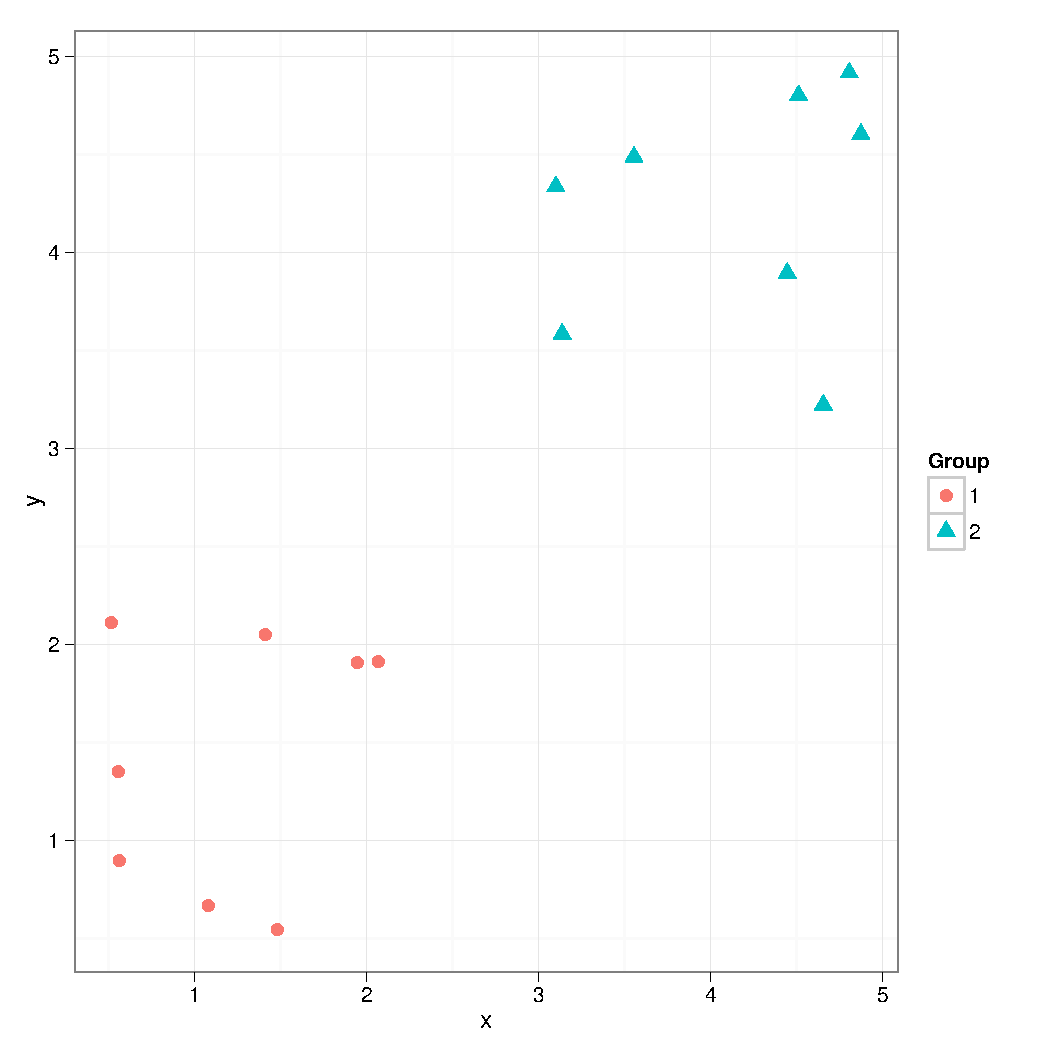
\includegraphics[width=10cm]{./plots/classification.pdf}
\subsection{Logistic hypothesis function}
\label{sec-3-2}


For logistic regression, we want a function that predicts into classes \(y=0\) or
\(y=1\). Because of this, the sigmoid function, \(y = \frac{1}{1 + e^{-\theta^T x}}\), is
typically used, which looks like this:



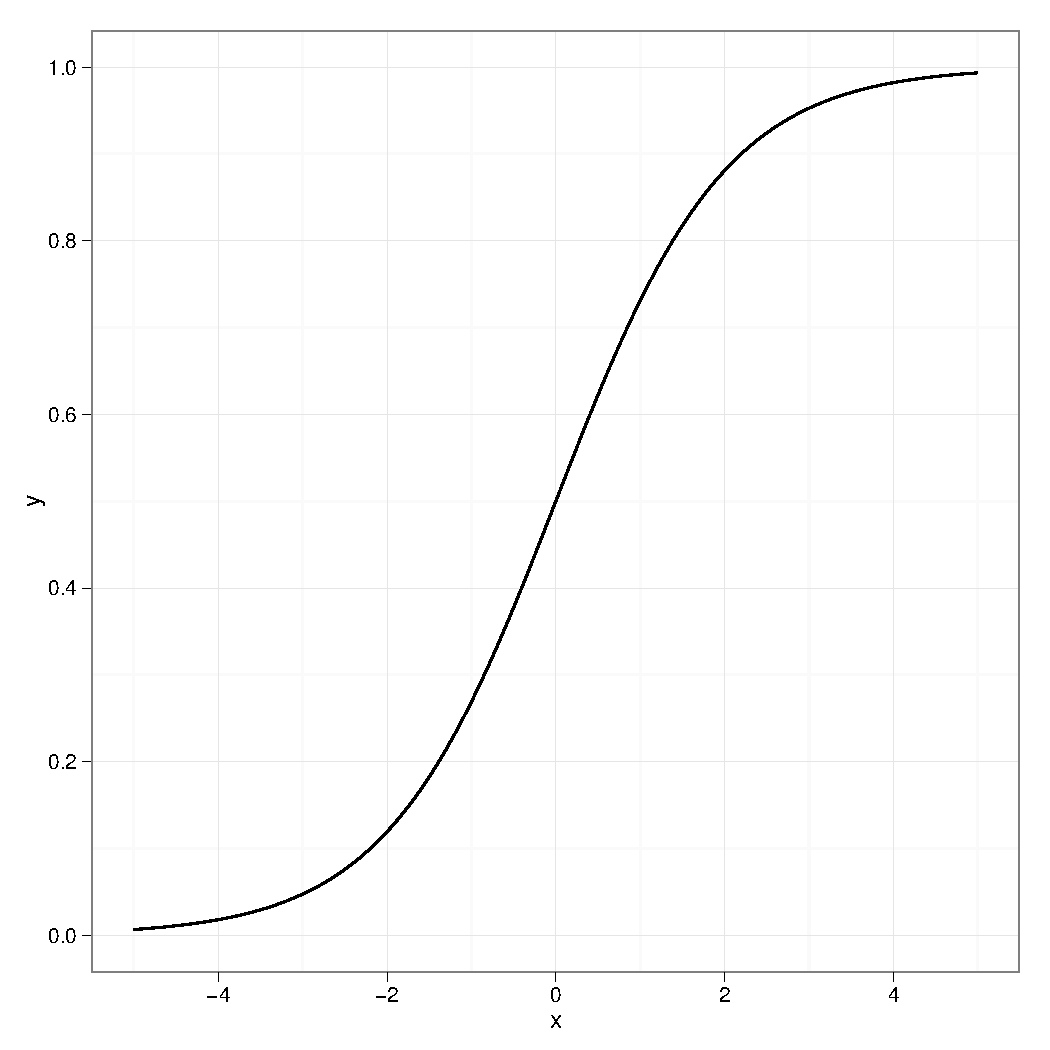
\includegraphics[width=10cm]{./plots/sigmoid.pdf}

In terms of a cost function, the mean squared error no longer works as we need to
cluster points in and out of a group, now determine their errors as measured by the
distance from points and our fitted line. The cost function \(J(\theta)\) used is as
follows:

\(
\begin{array}{l}
\textrm{for } y=1, J(\theta) = - ln(h(x)_\theta) \\
\textrm{for } y=0, J(\theta) = - ln(1 - h(x)_\theta) \\
\end{array}
\)

This can be re-written like so:
\[
J(\theta) = -y \; ln(h(x)_\theta) - (1-y) \; ln(1-h((x)_\theta))
\]

Thus, when either \(y=0\), or \(y=1\), we're left with the desired cost function. To
see why these are desirable functions, note this plot:



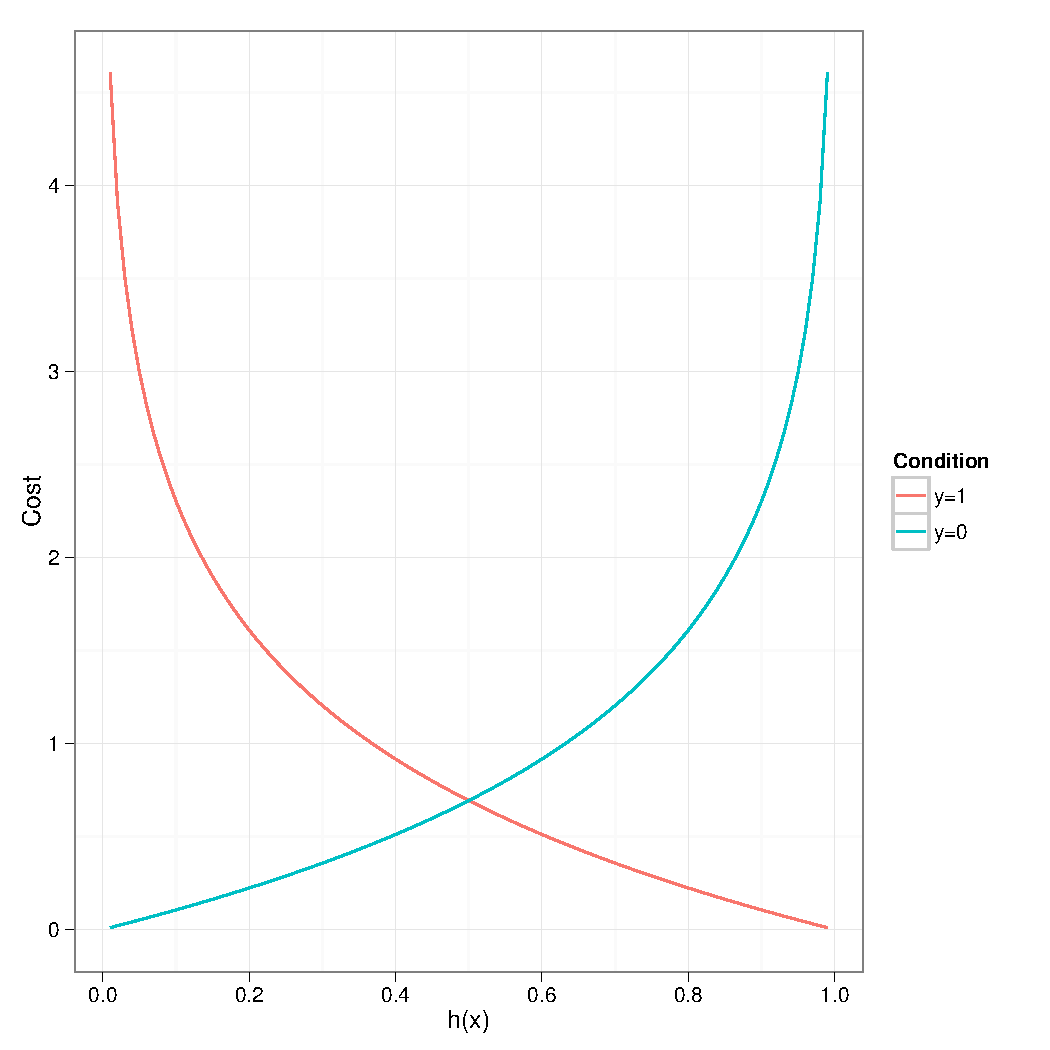
\includegraphics[width=10cm]{./plots/sigmoid-cost.pdf}

We choose this function for the following reason:

\begin{center}
\begin{tabular}{lll}
 Condition                      &  Actual value of \(y\)  &  Output of \(J(\theta)\)  \\
\hline
 \(h(x)_\theta \rightarrow 0\)  &                      0  &  0                        \\
 \(h(x)_\theta \rightarrow 1\)  &                      1  &  0                        \\
\hline
 \(h(x)_\theta \rightarrow 0\)  &                      1  &  \(\infty\)               \\
 \(h(x)_\theta \rightarrow 1\)  &                      0  &  \(\infty\)               \\
\end{tabular}
\end{center}



In other words, for correct predictions, the algorithm is not penalized, but for
highly erroneous predictions, the penalty approaches \(\infty\).
\subsection{Gradient descent for logistic regression}
\label{sec-3-3}

In order to apply gradient descent, we need to find the derivative of the cost
function. This is done in the following manner. We start with our cost function,
\(J(\theta)\): 
\[
J(\theta) = -y \; ln(h_\theta(x)) - (1-y) \; ln(1-h_\theta(x))
\]

Using the chain rule, we can break things up for both parameters of the equation:
\[
\frac{\partial}{\partial h_\theta(x)} J(h_\theta(x)) = \frac{\partial}{\partial
h_\theta(x)} g(h_\theta(x)) \frac{\partial}{\partial \theta^T} h_\theta(x)
\]

For the left side of the equation, we have:
\[
\frac{\partial}{\partial h_\theta(x)} -y \; ln(h_\theta(x)) = \frac{-y}{h_\theta(x)}
h'_\theta(x)
\]

For the right side, we have:
\[
\frac{\partial}{\partial h_\theta(x)} (1-y) \; ln(1 - h_\theta(x))
 = \frac{1 - y}{1 - h_\theta(x)}( -h'_\theta(x))
\]

To solve for the derivative of \(h'_\theta(x)\), it's helpful to rewrite it like so:
\(\frac{1}{1+e^{-\theta^T x}} = (1+e^{-\theta^T x})^{-1}\).

This way, we can write the derivative, again, in terms of the chain rule:
\[
\frac{\partial}{\partial (1+e^{-\theta^T x})}(1+e^{-\theta^T x})^{-1} \;
\frac{\partial}{\partial \theta^T} 1+e^{-\theta^T x}
\]

This becomes:
\[
-(1+e^{-\theta^T x})^{-2} \; (-xe^{-\theta^T x}) = \frac{xe^{-\theta^T
x}}{(1+e^{-\theta^T x})^2}
\]

And since \(h_\theta(x) = \frac{1}{1 + e^{-\theta^T x}}\) we see we can re-write the
above in terms of itself:
\[
-(1+e^{-\theta^T x})^{-2} \; (-xe^{-\theta^T x}) = x e^{-\theta^T x}
\frac{1}{1+e^{-\theta^T x}} \frac{1}{1+e^{-\theta^T x}} = x e^{-\theta^T x} \; (h_\theta(x))^2
\]

We can now substitute the definition of \(h'_\theta(x)\) into the partial derivatives
we found above:
\[
\frac{\partial}{\partial h_\theta(x)} J(\theta) = \frac{-y}{h_\theta(x)}
h'_\theta(x) - \left( \frac{1 - y}{1 - h_\theta(x)} h'_\theta(x) \right) = \frac{-y x e^{-\theta^T x} \; (h_\theta(x))^2}{h_\theta(x)} - \left( \frac{(1 - y)(-x
e^{-\theta^T x} \; (h_\theta(x))^2)}{1 - h_\theta(x)} \right)
\]

How to simplify this further? Using a clever observation:
\[
1-h_\theta(x) = 1 - \frac{1}{1+e^{-\theta^T x}} = \frac{1+e^{-\theta^T
x}}{1+e^{-\theta^T x}} - \frac{1}{1+e^{-\theta^T x}} = \frac{e^{-\theta^T
x}}{1+e^{-\theta^T x}} = e^{-\theta^T x}h_\theta(x)
\]

Now we can start cancelling things out:
\[
\frac{-y x e^{-\theta^T x} \; (h_\theta(x))^{\cancel{2}}}{\cancel{h_\theta(x)}} - \left( \frac{(1 - y)(-x
\cancel{e^{-\theta^T x}} \; (h_\theta(x))^{\cancel{2}})}{\cancel{e^{-\theta^T x}}
\cancel{h_\theta(x)}} \right) = \left (-y x e^{-\theta^T x} \; h_\theta(x)\right) -\left( (1 - y)(-x h_\theta(x))\right)
\]

Factoring out common terms and rearranging:
\[
-xh_\theta(x) (ye^{\theta^T x}-(1-y)) = -xh_\theta(x) (y(e^{\theta^T x}+1)-1)
\]

But \(1+e^{\theta^T x}\) is \((h_\theta(x))^{-1}\):
\[
-xh_\theta(x) (y(e^{\theta^T x}+1)-1) =
-x \left( \frac{y\cancel{h_\theta(x)}}{\cancel{h_\theta(x)}}-h_\theta(x) \right) =
\frac{1}{m} \sum_{i=1}^m \left( h_\theta(x^{(i)}) - y^{(i)} \right)x^{(i)}
\]
\subsection{Logistic regression for multiple classes}
\label{sec-3-4}

For multi-class problems, we can use something known as ``one vs. all''
classification. Instead of thinking of the problem as classifying into categories A,
B, C, and D, we create one hypothesis, \(h_\theta(x)^{(i)}\), per class which simply
predicts \(p(y = class | x; \theta)\). In other words, each hypothesis only examines
\(x\)'s with respect to the class of interest \(y = 1\). All other classes yield a
\(y=0\) result. After running each hypothesis, the classification of each training
example can be made with respect to the probability outputs of each
\(h_\theta(x)^{(i)}\).
\section{Week 3: Overfitting}
\label{sec-4}

An issue with both linear regression and logistic regression can occur when using
higher order fits to the data. Overfitting is more likely, which can result in
extremely low values for \(J(\theta)\), but unjustified contortions in the function
simply for the sake of minimizing cost.

With respect to terminology, an underfit function can be said to have high
bias. Fitting a curved data set with \(h_\theta(x) = \theta_0 + \theta_1 x_1\) is said
to be biased in that the function already assumes a linear relationship. Perhaps a
second order function fits the data reasonably well. Extending to third and fourth
order functions may achieve a minimum cost value, but also contain wild curves as the
function drives through the points.
\subsection{Regularization}
\label{sec-4-1}


A way to minimize overfitting is to include an extra term in the cost function:
\[
J(\theta) = \frac{1}{2m} \left [\sum_{i=1}^m \left( h_\theta(x^{(i)}) - y^{(i)} \right)^2 +
\lambda \sum_{j=1}^n \theta^2_j \right]
\]

By introducing this ``regularization term,'' we increase the cost function by \(\lambda
\theta^2_j\) and thus create a tension between minimizing error and keeping
\(\theta\)'s on the smaller side. As a side note \(\theta_0\) is not typically
penalized since it simply sets an intercept/baseline for the function. This is
particularly hepful for learning problems where \(n\) is very large. Perhaps we don't
want all \(n\) features to have a large role in determining the best hypothesis for
the given data, especially if we include higher order polynomials. For the housing
example, including a regularization term can help smooth out even a third and fourth
degree polynomial fit vs. risking wild curves for the sake of zero error.

While the idea is perhaps more easily grasped with respect to linear regression, the
same phenomenon can occur with logistic regression, where an overfit hypothesis will
make wild turns through the training example space to exclude any negative samples
and include all positive samples. Instead, we'd like the best fit ``approximate rule''
which is robust for future predictions even if it mis-classifies some of the current
training examples. Thus, regularization can simplify logistic regression as well.
\subsection{Regularization applied to linear regression}
\label{sec-4-2}


When finding the derivative for gradient descent, including the regularization
parameter, we end up with two update rules since we don't want to regularize
\(\theta_0\):

\( \displaystyle
\theta_0 := \theta_0 - \alpha \frac{1}{m} \sum_{i=1}^m \left( h_\theta(x^{(i)}) -
y^{(i)} \right)x^{(i)}_0 \\
\theta_j := \theta_j - \alpha \left[ \frac{1}{m} \sum_{i=1}^m \left( h_\theta(x^{(i)}) -
y^{(i)} \right)x^{(i)}_j + \frac{\lambda}{m} \theta_j \right]
\)

Factoring out the regularization term, we have:

\( \displaystyle
\theta_j := \theta_j(1 - \alpha \frac{\lambda}{m}) - \alpha \frac{1}{m} \sum_{i=1}^m \left( h_\theta(x^{(i)}) -
y^{(i)} \right)x^{(i)}_j
\)

\(1 - \alpha \frac{\lambda}{m}\) will always have the property of being \(< 1\),
since we're trying to reduce the influeince of the various \(\theta_j\)'s to avoid
overfitting.

Assuming we have a design matrix \(X\) and response matrix \(y\):

\( \displaystyle
X =
\begin{bmatrix}
1 & x^{(1)}_1 &  \cdots & x^{(1)}_n \\
1 & x^{(2)}_1 &  \cdots & x^{(2)}_n \\
\vdots & \vdots & \ddots & \vdots \\
1 & x^{(m)}_1 &  \cdots & x^{(m)}_n \\
\end{bmatrix} \qquad
y = 
\begin{bmatrix}
y^{(1)} \\
y^{(2)} \\
\vdots \\
y^{(m)} \\
\end{bmatrix}
\)

The linear regression normal equation states \( \displaystyle \theta = \left( X^T X
\right)^{-1} X^T y \). Adjusted for regularization, we now include \(\lambda\) times
a pseudo identity matrix where all by the first row has a 1 in the diagonal. This
matrix will have dimentions \((n+1) \times (n+1)\).

\( \displaystyle
\theta = \left( X^T X + \lambda
\begin{bmatrix}
0 & & & & \\
& 1 & & & \\
& & 1 & & \\
& & & \ddots & \\
& & & & 1 \\
\end{bmatrix}
\right )^{-1} X^T y
\)

With respect to non-invertability, \(X^T X\) will not be invertible for cases where
\( m <= n \), however in Octave, \texttt{pinv()} may still invert the matrix, but the
hypothesis may not be sound. It is possible to show that with the regularization term
included, the above adjusted normal equation will always be invertible.
\subsection{Regularization applied to logistic regression}
\label{sec-4-3}

Similar to the case of linear regression, we can adjust the cost function with the
same \( \lambda \) term:

\[
J(\theta) = - \left[ \frac{1}{m} \sum_{i=1}^m y \; ln \; h_\theta(x^{(i)}) + (1-y) \;
ln(1-h_\theta(x^{(i)})) \right] + \lambda \frac{1}{2m} \sum_{i=1}^n \theta^2_j
\]

Also, we end up with two separate updates for \( \theta_0 \) and \( \theta_{1
\rightarrow n} \):

\( \displaystyle
\theta_0 := \theta_0 - \alpha \frac{1}{m} \sum_{i=1}^m \left( h_\theta(x^{(i)}) -
y^{(i)} \right)x^{(i)}_0 \\
\theta_j := \theta_j - \alpha \left[ \frac{1}{m} \sum_{i=1}^m \left( h_\theta(x^{(i)}) -
y^{(i)} \right)x^{(i)}_j + \frac{\lambda}{m} \theta_j \right]
\)

\end{document}
